\documentclass[12pt]{article}
\usepackage[margin=1in, headheight=20pt]{geometry}
\usepackage{xcolor}
\usepackage{tikz}
\usepackage{eso-pic}
\usepackage{amsthm, amsmath, amssymb}
\usepackage{mathtools}
\usepackage[italicdiff]{physics}
\usepackage{enumitem}
\usepackage{lmodern}
\usepackage{fancyhdr}
\usepackage{pgfornament}
\usepackage{verbatim}
\usepackage{parskip}

\definecolor{pagecolor}{HTML}{DCE2F0}
\definecolor{textcolor}{HTML}{373D4A}

\pagecolor{pagecolor}
\color{textcolor}

\AddToShipoutPictureBG{
  \begin{tikzpicture}[remember picture, overlay]
    \draw[
      line width=0.5pt,
      color=textcolor,
      opacity=0.075
    ]
    (current page.south west) grid[step=10pt] (current page.north east);
  \end{tikzpicture}
}

\pagestyle{fancy}
\fancyhf{}
\fancyhead[L]{Computation of Option Pricing Models}
\fancyhead[R]{\nouppercase{\leftmark}}
\fancyfoot[C]{}

\renewcommand{\headrule}{
  \vspace{-5pt}
  \hbox to \headwidth{
    \leaders\hrule height 0.5pt\hfill
    \hspace{5pt}
    \raisebox{0.20pt}{\pgfornament[width=1cm]{11}}
    \hspace{5pt}
    \leaders\hrule height 0.5pt\hfill
  }
}

\renewcommand{\footrule}{
  \vspace{-12pt}
  \hbox to \headwidth{
    \leaders\hrule height 3.5pt depth -3pt \hfill 
    \hspace{5pt} 
    \thepage 
    \hspace{5pt}
    \leaders\hrule height 3.5pt depth -3pt \hfill
  }
}

\fancypagestyle{plain}{
  \fancyhf{}
  \renewcommand{\headrulewidth}{0pt}
  \renewcommand{\headrule}{} 
  \fancyfoot[C]{}
  \renewcommand{\footrule}{
    \vspace{-12pt}
    \hbox to \headwidth{
      \rule[0.65ex]{0.47\headwidth}{0.5pt}%
      \hfill
      \thepage
      \hfill
      \rule[0.65ex]{0.47\headwidth}{0.5pt}%
    }
  }
}

\newcommand{\bb}[1]{\mathbb{#1}}
\newcommand{\cl}[1]{\mathcal{#1}}

\newcommand{\p}[1]{\left ( #1 \right )}
\newcommand{\bk}[1]{\left [ #1 \right ]}
\newcommand{\br}[1]{\left \{ #1 \}}
\newcommand{\ab}[1]{\langle #1 \rangle}

\newcommand{\f}[2]{\frac{#1}{#2}}
\newcommand{\ety}{\varnothing}
\newcommand{\oo}{\infty}

\newcommand{\del}{\delta}
\newcommand{\gm}{\gamma}
\newcommand{\de}{\delta}
\newcommand{\De}{\Delta}
\newcommand{\ep}{\varepsilon}
\newcommand{\la}{\lambda}
\newcommand{\si}{\sigma}
\newcommand{\om}{\omega}
\newcommand{\Om}{\Omega}

\newcommand{\imp}{\Rightarrow}
\newcommand{\pmi}{\Leftarrow}
\renewcommand{\iff}{\Leftrightarrow}
\newcommand{\ffi}{\Rightarrow\!\Leftarrow}

\DeclareMathOperator{\Var}{Var}
\DeclareMathOperator{\std}{std}
\newcommand{\pd}{\partial}

% \renewcommand{\bar}[1]{\overline{#1}}

\newtheoremstyle{boldnote}
  {}
  {}
  {\itshape}
  {}
  {\bfseries}
  {.}
  { }
  {\thmname{#1}\thmnumber{ #2}\thmnote{ (\bfseries #3)}}
\theoremstyle{boldnote}
\newtheorem{theorem}{Theorem}[section]
\newtheorem{lemma}[theorem]{Lemma}
\newtheorem{corollary}[theorem]{Corollary}

\theoremstyle{definition}
\newtheorem{definition}[theorem]{Definition}
\newtheorem{example}[theorem]{Example}
\newenvironment{solution}
  {\begin{proof}[Solution]}
  {\renewcommand{\qedsymbol}{$\blacksquare$}\end{proof}}

\title{
    \textbf{Computation of Option Pricing Models}
}
\author{
  Dhyan Laad \\
  \texttt{2024ADPS0875G}
}
\date{}

\begin{document}
\maketitle
\tableofcontents
\newpage
\begin{comment}
\section{Preliminaries}
\subsection{Terminology}
\begin{definition}
    An \emph{option} is a financial derivative that grants the holder the right, but not the obligation to engage in a financial transaction with the underlying asset. A \emph{call option} is the right to buy the underlying asset while the \emph{put option} is the right to sell the underlying asset. A \emph{European option} can only be exercised exactly at expiration date, while an \emph{American option} can be exercised at any stopping time until the expiration date.
\end{definition}

\begin{definition}
    The \emph{stock price} or \emph{asset price} (denoted $S_t$) is the value of the underlying asset at a specific time $t$. It is modelled as a stochastic process adapted to a filtration.
\end{definition}

\begin{definition}
    The \emph{strike price} or \emph{exercise price} (denoted $K$) of a financial contract is a fixed, pre-determined price at which the holder of a derivative contract can exercise their right to buy or sell the underlying asset.
\end{definition}

\begin{definition}
    The \emph{duration} is the remaining lifespan of an option. If the maturity date is $T$, and the current time is $t$, then the duration is defined as $\tau = T - t$.
\end{definition}

\begin{definition}
    The \emph{volatility} (denoted $\si$) of a stock is a measure of its uncertainty. If $\De t$ is an arbitrary difference in two times, then the standard deviation of the stock's return in that time difference is given by $\si\sqrt{\De t}$.
\end{definition}

In addition to these parameters, an option's price is also affected by the risk-free interest rate $r$, and the dividends paid $q$.

\subsection{Market Assumptions}
\subsubsection{Principle of No Arbitrage}
In essence the Principle of No Arbitrage stipulates that instant risk-free profit should be impossible, often encapsulated in the saying ``there is no such thing as a free lunch."

\subsubsection{Efficient Market Hypothesis}
The Efficient Market Hypothesis (EMH) stipulates that an asset's current price fully reflects all available information. Consequently, knowing the historical path of the price provides no advantage in predicting its future movements. This implies that the future evolution of the asset depends solely on its current state, allowing us to model the price as a Markov process.
\end{comment}

\section{Fundamentals of Option Pricing}
Recall that a European put option gives its holder (buyer) the right, but not the obligation, to \emph{sell} a prescribed asset $S$ to the writer (seller) of the option for a strike price $K$ at the maturity date $T$. As such, the fair price $P$ of a European put option at the maturity date is simply given by the payoff:
\[P_T = P(S_T, T) = \max (K - S_T, 0).\]

Similarly, a European call option gives its holder the right, but not the obligation, to \emph{buy} a prescribed asset $S$ from the writer of the option, and once again fair price $P$ of a European call option at the maturity date is given by the payoff:
\[C_T = C(S_T, T) = \max (S_T - K, 0).\]

The objective of option pricing is to determine the value of \emph{premium}:
\[P_0 = P(S_0, 0), \quad C_0 = C(S_0, 0)\] 
building on the values of $P_T$. If $P_0$ was simply set to $0$ (no premium on the option), then a call option holder would never take on any risk, and never make a loss. On the other hand, the writer can never turn a profit. The price of the premium must be \emph{fair} to both parties entering the contract.

An investor is said to have taken the \emph{long position} if he/she has bought the option, and the \emph{short position} if he/she has sold the option.

Our models pretend that we are in a risk-neutral world, where an investor wouldn't mind risk. In this hypothetical world, a risky stop is expected to grow at the exact same rate as a safe investment such as a government bond or a bank account. The \emph{Risk-Neutrality Assumption} is as stated.
\begin{center}
  \emph{At any time, the average return on a risky investment of an asset is equal to the return on a risk-free investment of that asset.}
\end{center}

Under this new assumption,
\[E(P_T) = P_0e^{rT}.\]
And therefore the premium for a European call option would be
\[P_0 = e^{-rT}E(\max(S_T-K, 0)).\]

\subsection{Modelling a Risk-Free Asset}
A bond issued by the government, or accumulating interest in a bank can be regarded as a risk-free asset. If $B_0$ is a risk-free investment at a time $t = 0$, the value of the investment after $m$ years at a rate $r$ would be
\[B_m = B_0(1 + mr)\]
if the interest is simple, and
\[B_m = (1 + r)^mB_0\]
if compounded anually. Building on the case of compound interest, consider $N$ timestamps $\{t_n : n \in 0 : N\}$ where $t_n = n \del t = n/N$ at which the interest compounds. Then,
\[\f{B_{t_n} - B_{t_{n-1}}}{B_{t_{n-1}}} = r\del t\]
for $n \in 1 : N$. Now,
\[B_T = B_{t_N} = (1 + r\del t)^NB_0 = [(1 + r\del t)^{1/\del t}]^TB_0.\]
If the interest is compounded continuously, then
\[B_T = \lim_{\del t \to 0} [(1 + r\del t)^{1/\del t}]^TB_0 = e^{rT}B_0.\]

\subsection{Call-Put Parity}
The call-put parity is a relation between a European call option, put option, and its underlying asset. Consider the following portfolio $\Pi$, consisting of one long put $P$ and short call $C$, both with the same strike price $K$ and expiration date $T$ and one underlying asset $S$:
\[\Pi = S + P - C.\]
The payoff for this portfolio at maturity is always fixed:
\[S_T + \max (K-S_T, 0) - \max(S_T - K, 0) = K.\]
To determine how much one should pay for $\Pi$, we simply discount the risk-free interest (at rate $r$) gained from $K$:
\[\Pi = Ke^{-r(T - t)} \imp S + P - C = Ke^{-r(T-t)}.\]
This final equation is called the call-put parity relation.

If one were to introduce a stock that pays dividends $D$, the relation becomes
\[S + P = C + D + Ke^{-r(T-t)}.\]

\subsection{Assumptions in Asset Pricing}
The basic principle of asset pricing is that the value of an asset cannot be predicted, since it is a measure of investors' confidence, and as such, is strongly dependent on news, rumours, speculation, and general human behaviour. For the sake of mathematical simplification, we assume that the market responds instantenously to external influence. This is captured in the \emph{Efficient Market Hypothesis} (EMH) described below.

\begin{enumerate}
  \item \emph{The past history of an asset is fully reflected in its present price.}
  \item \emph{The market responds immediately to any new information about an asset.}
\end{enumerate}

Based on the first principle, asset prices are modelled with Markov processes.

In addition to the EMH, a number of assumptions are made about the asset, as listed.
\begin{itemize}
  \item The asset price may take any nonnegative value.
  \item Buying and selling an asset may take place at any time $t \in [0, T]$
  \item It is possible to buy and sell any amount of the asset.
  \item The bid-ask spread is zero: the price for buying an asset equals the price for selling it.
  \item There are no transaction costs.
  \item There are no dividends or stock splits.
  \item Short-selling is permitted: it is possible to hold a negative amount of the asset.
  \item There is a single, constant, risk-free interest rate that applies to any amount of money borrowed from or deposited in a bank.
\end{itemize}

\section{Fundamentals of Probability Theory}

\subsection{Measure Theoretic Foundations}
\begin{definition}
  A nonempty collection $\cl A$ of subsets of a nonempty set $\Om$ is said to be a \emph{$\si$-algebra on $\Om$} if it satisfies the following assumptions.
  \begin{enumerate}
    \item $A \in \cl A \imp A^c \in \cl A$.
    \item If $\{A_i\}$ is a sequence of sets in $\cl A$, then
    \[\bigcup_{i=1}^\oo A_i \in \cl A.\]
  \end{enumerate}
\end{definition}

It follows from these axioms that $\Om, \ety \in \cl A$, and $\cl A$ is closed under countable intersections as well due to De Morgan's rules:
\[\bigcap_{i=1}^\oo A_i = \p{\bigcup_{i=1}^\oo A_i^c}^c \in \cl A \]
for some sequence $\{A_i\}$ in $\cl A$.

The pair $(\Om, \cl A)$ is called a \emph{measurable space}.

\begin{definition}
  The \emph{Borel $\si$-algebra} of $\bb R$ denoted $\cl B(\bb R)$ is the smallest $\si$-algebra that contains all open sets in $\bb R$. All intervals, singleton subsets, and countable sets are contained in the Borel $\si$-algebra, and are called \emph{Borel sets}.
\end{definition}

\begin{definition}
  A set function $P : \cl A \to [0,1]$ is known as a \emph{probability measure} on a measurable space $(\Om, \cl A)$ if it satisfies the following assumptions.
  \begin{enumerate}
    \item $P(\ety) = 0$ and $P(\Om) = 1$.
    \item For a sequence of sets $\{A_i\}$ which are pairwise disjoint,
    \[P\left (\bigcup_{i=1}^\oo A_i \right ) = \sum_{i=1}^\oo P(A_i)\]
  \end{enumerate}
\end{definition}

Now the tuple $(\Om, \cl A, P)$ is called a \emph{probability space}.

We may now define random variables and stochastic processes.

\begin{definition}
  A real valued \emph{random variable} $X$ on a probability space $(\Om, \cl A, P)$ is a $\cl A$-measurable real valued function on $\Om$. That is, for every $B \in \mathcal B (\bb R)$, it follows that $X^{-1}(B) \in \cl A$.
\end{definition}

A random variable can be viewed as a useful tool for transitioning from an abstract probability space $(\Om, \cl A, P)$, to a more tangible one on the real numbers: $(\bb R, \cl B(\bb R), P_X)$. Here $P_X$ is called a \emph{push-forward measure}. For any $B \in \cl B(\bb R)$,
\[P_X(B) = P(X^{-1}(B)).\]

\begin{definition}
  A real valued \emph{stochastic process} $\{X_t\}$ on a probability space $(\Om, \cl A, P)$ assigns to each time $t$ from a set $T$, a random variable $X_t$ on $(\Om, \cl A, P)$. The process $X_t$ has \emph{a.s.} continuous sample paths $t \mapsto X_t(\om)$.
\end{definition}

We will drop the braces around $\{X_t\}$, and refer to $X_t$ as a stochastic process for brevity.

\begin{definition}
  A \emph{discrete random variable} $X$ takes values from a finite set of numbers $\{x_1, x_2, \dots , x_m\}$ and associates these with probabilities $\{p_1, p_2, \dots , p_m\}$ such that $x_i$ occurs with probability $p_i$. Symbolically,
  \[P(X = x_i) = p_i.\]
\end{definition}

\subsection{Expectation and Independence}

\begin{definition}
  Let real valued $X$ be a random variable on a probability space $(\Om, \cl A, P)$. The \emph{expected value} or \emph{expectation} of $X$ is given by
  \[E(X)= \int_\Om X(\om)\dd{P(\om)}.\]
\end{definition}

The definition of expectation provided above is the most general one, and from it one can derive the familiar definitions from elementary probability. For the case of a discrete random variable $X$ taking on values $\{x_1, x_2, \dots , x_n\}$,
\[X(\om) = \sum_{i=1}^n x_i \vb 1_{A_i}(\om)\]
where $A_i = \{\om \in \Om : X(\om) = x_i\}$. Plugging this into our definition for expected value,
\[E(X) = \int_{\Om} \p{\sum_{i=1}^n \vb 1_{A_i}(\om)}\dd{P(\om)} = \sum_{i=1}^n x_i \int_{\Om} \vb 1_{A_i}(\om)\dd{P(\om)} = \sum_{i=1}^n x_iP(X = x_i).\]

In the case that $X$ is a continuous random variable, we may switch to integrating over $\bb R$ instead:
\[E(X) = \int_\Om X(\om)\dd{P(\om)} = \int_{\bb R} x\dd{P_X(x)}.\]
Using the Radon-Nikodym theorem with the Lebesgue measure, we know that there exists a derivative function $f$ such that $\dd{P_X} = f\dd{x}$. As such,
\[\int_{\bb R}x\dd{P_X(x)} = \int_{\bb R}xf(x)\dd{x}.\]

The expectation of $g(X)$ for an any function $g$ that is Borel measurable and absolutely integrable with respect to $f$ is given by
\[E(g(X)) = \int_{\bb R} g(x)f(x)\dd{x}.\]
Note that $P(X \in A) = E(\vb 1_A(X))$, therefore:
\[P(X \in A) = \int_{\bb R} \vb 1_A(x)f(x)\dd{x} = \int_A f(x)\dd{x}.\]
For the case that $A$ is an interval $(a, b]$:
\[P(a < X \leq b) = \int_a^b f(x)\dd{x}.\]

The operator $E$ is linear. That is, for two random variables $X$ and $Y$, and $a \in \bb R$,
\[E(X + aY) = E(X) + aE(Y).\]

We now look at another important property: independence.

\begin{definition}
  Two random variables $X$ and $Y$ are said to be \emph{independent} if for all Borel measurable functions $g, h \in \bb R^{\bb R}$,
  \[E(g(X)h(Y)) = E(g(X))E(h(Y)).\]
\end{definition}

\begin{definition}
  A set of random variables $\{X_1, X_2, \dots , X_n\}$ are sad to be \emph{indepdently and identitcally distributed} or i.i.d. if 
  \begin{enumerate}[label=(\alph*)]
    \item for discrete random variables, every $X_i$ for $i \in 1 : n$ has the same set of possible outcomes and same probability for each outcome, and the same density for continuous random variables, and
    \item the outcome of one variable provides no information on the others.
  \end{enumerate}
\end{definition}

We now proceed to define variance, a measure of the amount of variation around around the mean.
\begin{definition}
  For a random variable $X$ such that $E(X^2) < \oo$, its \emph{variance} is defined as
  \[\Var(X) = E((X - E(X))^2).\]
\end{definition}

It can be expanded as
\[\Var(X) = E(X^2) - E(X)^2.\]

It also holds that $\Var(aX) = a^2\Var(X)$ for all $a \in \bb R$, and the \emph{standard deviation} is defined as the square root of the variance: $\std(X) = (\Var(X))^{1/2}$.

\subsection{The Wiener Process}

We now proceed to define the normal distribution, which is central to our study.
\begin{definition}
  If $X$ is a continuous random variable with density function $f : \bb R \to \bb R$ such that
  \[f(x) = \f{1}{\sqrt{2\pi \si^2}}\exp \p{- \f{(x - \mu)^2}{2\si^2}}\]
  where $\mu, \si \in \bb R$ with $\si > 0$, then we say that $X$ has a \emph{normal distribution} or is \emph{normally distributed}. The parameters $\mu$ and $\si^2$ are the mean and variance of the distribution respectively, and we symbolically write
  \[X \sim \cl N(\mu, \si^2).\]
\end{definition}

We recover the standard normal distribution for $\mu = 0$ and $\si = 1$.

\begin{definition}
  If $X$ is a continuous random variable such that $\log X \sim \cl N(\mu, \si^2)$ for constants $\mu, \si \in \bb R$ where $\si > 0$, then $X$ is said to be \emph{lognormally distributed} or have a \emph{lognormal distribution}. 
\end{definition}

\begin{definition}
  Given a density function $f$ for a continuous random variable $X$, the \emph{cumulative distribution function} (cdf) $F : \bb R \to \bb R$ of $X$ is given by
  \[F(x) = P(X \leq x) = \int_{-\oo}^x f(t)\dd{t}.\]
\end{definition}

The cdf of the standard normal distribution is of interest to us, and we denote it with $\Phi$:
\[\Phi(x) = \f{1}{\sqrt{2\pi}}\int_{-\oo}^x e^{-t^2/2}\dd{t}.\]

We may now proceed to define a Wiener process.
\begin{definition}
  A \emph{Wiener process} or \emph{Brownian motion} in one dimension is a stochastic process $W_t$ where $t \geq 0$ with the following properties.
  \begin{enumerate}
    \item $W_0 = 0$ \emph{a.s.}
    \item $W_t$ has independent increments: for every $t > 0$ and $\De t \geq 0$, $\De W_t = W_{t + \De t} - W_t$ is independent of $W_s$ for every $s < t$.
    \item $W_t$ has Gaussian increments: for every $t > 0$ and $\De t \geq 0$, $\De W_t = W_{t + \De t} - W_t \sim \cl N(0, \De t)$.
    \item $W_t$ is \emph{a.s.} continuous in $t$.
  \end{enumerate}
\end{definition}
We will reserve the notation $W_t$ for a Weiner process henceforth, without explict declaration.

The following properties hold for a Wiener process $W_t$. For $\De W_t = W_{t + \De t} - W_t$ where $t > 0$ and $\De t \geq 0$,
\begin{enumerate}[label=(\alph*)]
  \item $E(\De W_t) = 0$, and
  \item $\Var(\De W_t) = \De t$ implying that $\std(\De W_t) = \sqrt{\De t}$.
\end{enumerate}

In fact, $\De W_t = \ep \sqrt{\De t}$ where $\ep$ is drawn from a standard normal distribution. The heuristic that $\dd{W_t} \approx \sqrt{\dd{t}}$ may be drawn from this. We define a generalized Weiner process $\tilde{W}_t$ with a drift rate $r$ and volatility $\si$:
\[\dd{\tilde{W}_t} = r\dd{t} + \si \dd{W_t} \imp \tilde{W}_t = \tilde{W}_0 +  rt + \si W_t.\]
This should be viewed as a specific case of an It\^o drift-diffusion process $X_t$ that satisfies the stochastic differential equation
\[\dd{X_t} = \mu_t\dd{t} + \si_t\dd{W_t}.\]

\section{Modelling Asset Prices}

\subsection{The Stochastic Differential Equation}
Asset prices follow stochastic processes. Let $\mu$ be the expected rate of return of a risk free ($\si = 0$) asset $S$. The asset price can be modelled as
\[\f{\dd{S_t}}{S_t} = \mu t.\]
This is a deterministic differential equation with solution
\[S_t = S_0e^{\mu t}.\]

We now attempt to model assets that have risk involved $(\si > 0)$. Returns from the asset come from two sources: the risk free rate interest rate governed by $\mu$, and the random changes due to the EMH, which we model with a Weiner process on some probability space $(\Om, \cl A, P)$. As such, we arrive at the stochastic differential equation:
\[\f{\dd{S_t}}{S_t} = \mu \dd{t} + \si\dd{W_t}.\]
This is called a \emph{geometric Brownian motion}. The notation is mathematically meaningless when written with differentials ($\dd{W_t} = W'_t\dd{t}$ doesn't really exist) and is better written as in integral equation, and we switch notation from $S_t$ to $S(t)$ to emphasize the path function for a fixed $\om \in \Om$.
\[S(t) = S_0 + \mu \int_0^t S(\tau)\dd{\tau} + \si \int_0^t S(\tau)\dd{W_{\tau}}.\]

These integrals exist \emph{a.s.} with the first one being a standard Riemann integral, and the second integral being a well-defined \emph{It\^o integral}.

\begin{example}
  For an asset $S$ that pays no dividends, has a volatility of $30$\% per annum, and provides an expected return of $15$\% per annum with continuous compounding interest, determine the return $\De S/S$ after a week ($0.0192$ years, since a working year is 250 days). Also find the mean and variance of $\De S$ when the asset price is $100$.
\end{example}
\begin{solution}
  Given that $\mu = 0.15$, and $\si = 0.30$, the return would be
  \[\f{\De S}{S} = 0.15\De t + 0.30 \De W.\]
  We know that $\De W = \ep \sqrt{\De t}$ where $\ep \sim \cl N(0, 1)$, and $\De t = 0.0192$. Therefore, the return would be
  \[\f{\De S}{S} = 0.00288 + 0.041\ep.\]
  
  Solving for $\De S$ at $S = 100$, we have
  \[\De S = 0.288 + 4.16\ep.\]
  Therefore,
  \[E(\De S) = 0.288 \quad \text{and} \quad \Var(\De S) = 4.16^2 = 17.31.\]
\end{solution}

An asset's expected return rate and volatility is rarely known to us, and must be estimated. Given an asset price $S$ at $n+1$ equal time steps $\De t$ $\{S_0, S_1, \dots , S_n\}$ in chronological order, we may estimate the expected rate of return
\[\bar{\mu} = \f{1}{n \De t} \sum_{i=0}^n \f{S_{i+1} - S_i}{S_i},\]
and the historical volatility is defined as the square root of the sample variance given by
\[\bar{\si}^2 = \f{1}{(n-1)\De t} \sum_{i=0}^{n-1} \p{\f{S_{i+1} - S_i}{S_i - \bar{\mu}}}^2.\]
Historical volatility is not a useful metric for our models. More sophisticated methods for estimating the volatility will be discussed later.

\subsection{It\^o's Lemma}
It\^o's lemma can be viewed as the stochastic equivalent of the chain rule from naive calculus. We explore a specific case of it here, relevant to option pricing.

Let $S_t$ be a geometric Brownian motion
\[\dd{S_t} = \mu S_t\dd{t} + \si S_t \dd{W_t}\]
and $f : [0, T) \times \bb R^+ \to \bb R$ a twice-differentiable scalar function. Using its Taylor series expansion, we have
\begin{align*}
  \dd{f} &= f(t + \dd{t}, S + \dd{S}) - f(t, S) \\
  &= \pdv{f}{t}\dd{t} + \pdv{f}{S}\dd{S} + \f 12 \p{{\pdv[2]{f}{t}}(\dd{t})^2 + 2\pdv[2]{f}{t}{S} \dd{t}\dd{S} + {\pdv[2]{f}{S}}(\dd{S})^2} + \cdots
\end{align*}
From the It\^o drift-diffusion equation, we know that
\[(\dd{S})^2 = (\mu S_t \dd{t} + \si S_t \dd{W_t})^2 = \mu^2S_t^2(\dd{t})^2 + 2\mu\si S_t^2 \dd{t}\dd{W_t} + \si^2S_t^2(\dd{W_t})^2.\]
We may now use the heuristic $\dd{W_t} \approx \sqrt{\dd{t}}$. Retaining terms that are atmost $O(\dd{t})$ (if any larger, they shrink too fast to be nonnegligible as $\dd{t} \to 0$), we obtain
\[\dd{f} = \p{\mu S \pdv{f}{S} + \pdv{f}{t} + \f 12 \si^2 S^2\pdv[2]{f}{S}}\dd{t} + \si S\pdv{f}{S}\dd{W_t}.\]
This statement is the version of It\^o's lemma we will be using.

It\^o's lemma can be extended to higher dimensions. If $\vb S_t = [S^1_t \; S^2_t \; \cdots \; S^n_t]^\top$ is a vector of It\^o drift diffusion processes, then
\[\dd{\vb{S}_t} = \boldsymbol{\mu}_t\dd{t} + \vb{G}_t\dd{\vb{W}_t}\]
for a vector $\boldsymbol{\mu}_t$ and matrix $\vb{G}_t$. This version of It\^o's lemma is called the Kunita-Watanabe lemma:
\[\dd{f} = \p{\pdv{f}{t} + (\grad_{\vb S} f)^\top \boldsymbol{\mu}_t + \f 12 \tr (\vb G_t^\top (H_{\vb S} (f))\vb G_t)}\dd{t} + (\grad_{\vb S} f)^\top \vb{G}_t\dd{\vb W_t}.\]


\subsection{Solution to the Stochastic Differential Equation}
Armed with It\^o's lemma, we may now attempt to solve the stochastic differential equation that models an asset's price:
\[\dd{S_t} = \mu S_t\dd{t} + \si S_t\dd{W_t}.\]

Apply It\^o's lemma on $f(t, S) = \log S$:
\begin{align*}
  \dd{(\log S_t)} &= \p{\mu S \p{\f 1S} + 0 + \f 12 \si^2 S^2 \p{-\f 1{S^2}}}\dd{t} + \si S \p{\f 1S} \dd{W_t} \\
  &= \p{\mu - \f 12 \si^2}\dd{t} + \si \dd{W_t}.
\end{align*}
This is an equation representing the previously described generalized Brownian motion; the solution to which can be obtained by ``integrating":
\[\log S_t = \log S_0 + \p{\mu - \f 12 \si^2}t + \si W_t.\]
Exponentiating we get,
\[S_t = S_0 \exp \p{\p{\mu - \f 12 \si^2}t + \si W_t}.\]

Since $W_t \sim \cl N(0, t)$, it follows that
\[\log S_t \sim \cl N \p{\log S_0 + \p{\mu - \f 12 \si^2}t, \si^2t}.\]
As such, $S_t$ is lognormally distributed.

Due to the lognormal distribution of $S_t$, we measure returns in a complimentary structure. The \emph{daily log-return} of the stock $S_t$ is defined as
\[r_t = \log \p{\f{S_t}{S_{t-1}}}.\]
where $t$ is measured in days. Given $n$ log returns $r_i$ for $i \in 1 : n$, the sample mean is defined as
\[\bar{r} = \f 1n \sum_{t=1}^n r_t\]
and sample variance
\[\hat{\si}^2_{\mathrm{daily}} = \f 1{n-1}\sum_{t=1}^n (r_t - \bar{r})^2,\]
the square root of which is the daily volatility.

Indian equity markets have approximately 252 trading days a year, and the \emph{annualized volatility} is
\[\hat{\si}_{\mathrm{annual}} = \sqrt{252}\hat{\si}_{\mathrm{daily}}.\]

The \emph{rolling volatility} calculates the volatility of an asset's price movements over a specified period. It measures the degree of variation in the price series over time, and provides insights into the market's potential price fluctuations. For a window of size $m$,
\[\hat{\si}_t = \sqrt{252}\std\{r_{t-m+1}, r_{t-m+2}, \dots r_t\}.\]

\section{Partial Differential Equations}

\subsection{Deriving the Black-Scholes Equation}
We now proceed to derive the Black-Scholes equation, the solution to which is the basis for models for fair option pricing. Recall the geometric brownian motion stochastic differential equation that governs stock trends:
\[\dd{S_t} = \mu S \dd{t} + \si S \dd{W_t},\]
and let $V \in C^{1, 2}([0, T) \times \bb R^+)$ be the price of an option depending on the time $t \in [0, T)$ and asset price $S_t \in \bb R^+$.

Using It\^o's lemma:
\[\dd{V} = \p{\pdv{V}{t} + \mu S \pdv{V}{S} + \f 12 \si^2 S^2 \pdv[2]{V}{S}} \dd{t} + \si S \pdv{V}{S}\dd{W_t}.\]
We now define a portfolio $\Pi$:
\[\Pi(t) = V(t, S(t)) - \De S(t),\]
where $\De$ is the number of assets held. The goal of the choice portfolio is to find a suitable value of $\De$ such that the randomness due to $\dd{W_t}$ is eliminated. We assume the portfolio is \emph{self-financing}:
\[\dd{\Pi} = \dd{V} - \De \dd{S}.\]
That is to say, all changes are financed internally. Substuting our values of $\dd{V}$ and $\dd{S}$ into the above equation,
\[\dd{\Pi} = \p{\pdv{V}{t} + \mu S \pdv{V}{S} + \f 12 \si^2 S^2 \pdv[2]{V}{S}} \dd{t} + \si S \pdv{V}{S}\dd{W_t} - \De (\mu S \dd{t} + \si S \dd{W_t}).\]
The coefficient of $\dd{W_t}$ is given by
\[\si S \pdv{V}{S} - \De \si S.\]
We may eliminate the stochastic part of the equation by simply setting this to $0$:
\[\De = \pdv{V}{S}.\]
The equation is now entirely deterministic:
\[\dd{\Pi} = \p{\pdv{V}{t} + \f 12 \si^2 S^2 \pdv[2]{V}{S}}\dd{t}\]
We now appeal to the principle of no arbitrage. If the same portfolio value was invested in a risk-free manner at rate $r$, we have
\[\dd{\Pi} = r\Pi \dd{t}.\]
From our now chosen value of $\De$, we have
\[\Pi = V - S\pdv{V}{S},\]
and obtain
\[\pdv{V}{t} + \f 12 \si^2 S^2 {\pdv[2]{V}{S}} = r\p{V - S \pdv{V}{S}}. \]
Rearranging, we get the Black-Scholes partial differential equation:
\[\pdv{V}{t} + \f 12 \si^2 S^2 {\pdv[2]{V}{S}} + rS\pdv{S}{V} - rV = 0,\]
along with the terminal condition
\[V(T, S_T) = \Phi(S_T) = \begin{cases}
  \max(S_T - K, 0) & \text{European call}, \\
  \max(K - S_T, 0) & \text{European put}.
\end{cases}\]

It is interesting to observe that the drift $\mu$ disappears from the equation, and only the volatility $\si$ affects option prices. Pricing depends on hedging, not on the expected return.

\begin{definition}
  \emph{Hedging} is the practice of taking a position in one market to offset and balance against the risk adopted by assuming a position in a contrary or opposing market or investment. A \emph{hedge} is an investment position intended to offset potential losses or gains that may be incurred by a companion investment.
\end{definition}

\subsection{Introduction to Partial Differential Equations}
\begin{definition}
  The \emph{order} of a partial differential equation (PDE) is the total order of highest derivative the occurs in it.
\end{definition}

\begin{definition}
  A PDE is said to be \emph{linear} if it is linear in the unknown function and derivatives. A PDE that is not linear is called \emph{nonlinear}.
\end{definition}

Alternatively if $L$ is an operator for the PDE
\[L(u) = f,\]
then $L$ is linear if
\begin{enumerate}
  \item $L(u + v) = L(u) + L(v)$, and
  \item $L(tu) = t L(u)$ for a constant $t$.
\end{enumerate}

In order for a PDE to have a unique solution, additional conditions on the solution in the form of initial conditions or boundary conditions, or some combination thereof need to be imposed on the solution. A linear boundary value problem (BVP) or initial value problem (IVP) will have the PDE and the associated boundary or initial conditions linear.

\begin{definition}
  A \emph{well-posed problem} consists of a PDE and associated boundary or initial conditions and satisfies the Hadamard criteria.
  \begin{description}
    \item[Existence.] It has a solution.
    \item[Uniqueness] The solution is unique.
    \item[Continuous Dependence.] The solution depends continuously on the associated independent variables.   
  \end{description}
\end{definition}

We will restrict our study to well-posed problems.

\subsection{Classification of Second Order Partial Differential Equations}

Consier a general second order algebraic equation in two variables with real coefficients:
\[ax^2 + 2bxy + cy^2 + dx + ey + f = 0.\]

The nature of the curve in $\bb R^3$ plotted by the \emph{principal part} $P(x, y) = ax^2 + 2bxy + cy^2$ depends on the sign on $b^2 - ac$.
\begin{enumerate}[label=\arabic*.]
  \item If $b^2 - ac > 0$, the curve is \emph{hyperbolic}.
  \item If $b^2 - ac = 0$, the curve is \emph{parabolic}.
  \item If $b^2 - ac < 0$, the curve is \emph{elliptical}.
\end{enumerate}

With a suitable coordinate transformation $(x, y) \mapsto (X, Y)$ depending on the roots of $P(x, y) = 0$, the equation may be written in its \emph{normal form} or \emph{canonical form}, mimicing the standard equations of the conic sections on $\bb R^2$.

Now consider a second order linear PDE in two variables with constant and real coefficients:
\[au_{xx} + 2bu_{xy} + cu_{yy} + du_x + eu_y + fu + g = 0.\]
The nature of the PDE will be once again determined by the principal part $P(\pd_x, \pd_y)u$ where
\[P(\pd_x, \pd_y) = P\p{\pdv{}{x}, \pdv{}{y}} = a{\pdv[2]{}{x}} + 2b\pdv[2]{}{x}{y} + c{\pdv[2]{}{y}}.\]
The PDE would be \emph{hyperbolic} if $b^2 - ac > 0$, \emph{parabolic} of $b^2 - ac = 0$, and \emph{elliptic} if $b^2 - ac < 0$.
\end{document}